\section{Experiment 10H-I: physically coupled fitting and output-only covariance selection}
\label{sec:experiment10hi}

\paragraph{Purpose and controlled separation.}
The numerical repair in Experiment 10H-H produced repeatable staged fits, but
its nine independently fitted coefficients violated an exact bicycle identity.
Experiment 10H-I enforces that identity and distinguishes two questions.
Part A changes only the physical parameterization, retaining the inherited
process covariance to isolate model structure. Part B chooses the process-noise
scale using measured training outputs alone. Both parts use opened development
fleets 601--605, the same 200-sample records and 20/10 training/held-out client
split as 10H-H. Part A verifies exact measured-array SHA-256 agreement with
the archived 10H-H records. This is development evidence, not blind
confirmation. Seeds 591--600 and 611--620 remain sealed.

\paragraph{Eight coordinates and exact coupling.}
The positive physical coordinates are
\begin{equation}
 w=(g,\ell_f,\ell_r,b_f,b_r,d_f,d_r,a_\delta),\qquad
 g=\frac{m}{I_z},\quad b_j=\frac{C_j}{m\sigma_j},\quad
 d_j=\frac{1}{\sigma_j},\quad a_\delta=\frac{1}{\tau_\delta}.
\end{equation}
Their physical definitions specify the model; true client values are not
inputs to estimation. The existing nine coefficients become
\begin{equation}
 \varphi(w)=
 (g\ell_f,g\ell_r,b_f,\ell_f b_f,b_r,\ell_r b_r,d_f,d_r,a_\delta).
 \label{eq:10hi-map}
\end{equation}
Equation~\eqref{eq:10hh-physical-coupling} therefore holds identically.
The relation reduces the physically admissible coefficient space from nine
to eight dimensions.
It does not identify absolute mass, inertia, or cornering stiffnesses:
common scaling of $m,I_z,C_f,C_r$ leaves the measured-output model unchanged.
Positive coordinates and this coupling ensure realizability in the adopted
bicycle structure, not that every feasible geometry represents a passenger
vehicle with plausible dimensions.

Let $\eta=\log(w/w_{\mathrm{nom}})$, where the nominal design is public.
Products in \eqref{eq:10hi-map} imply a constant full-column-rank map
\begin{equation}
 z=z_{\mathrm{nom}}+T\eta,\qquad
 \nabla_\eta\mathcal L=T^\top\nabla_z\mathcal L,\qquad
 \mathcal I_8=T^\top\mathcal I_9 T.
\end{equation}
The nine coefficient bounds are preserved exactly as
\begin{equation}
 z_{\mathrm{lower}}-z_{\mathrm{nom}}
 \le T\eta\le
 z_{\mathrm{upper}}-z_{\mathrm{nom}},
 \label{eq:10hi-bounds}
\end{equation}
with the existing 0.35--3.0 nominal multipliers. Independent boxes on the
eight new quantities would change the comparison and are not introduced.
Starts use the nominal and two deterministic perturbations in eight log
coordinates. A perturbation is shrunk along its nominal-centered ray until
all nine inequalities are satisfied. Coefficient-wise clipping is avoided
because it would break the physical identity.

\paragraph{Likelihood, optimization, and diagnostics.}
The repaired covariance, exact discretization, complete analytic derivatives,
and working likelihood in \eqref{eq:10hh-likelihood} are unchanged.
Training-only diagonal information scaling is calculated in the eight
coordinates. SLSQP handles the linear inequalities with analytic gradients.
Part A compares joint and staged fitting. Stages fit the actuator, relaxation
rates, and the five mechanical quantities, followed by joint refinement.
Restricted stages have 80 iterations and final joint optimization has 300,
with function tolerance $10^{-12}$ and three starts.

An independent KKT audit fits nonnegative multipliers to the outward normals
of active coefficient constraints. It reports stationarity, feasibility, and
complementarity in physical log coordinates. A box projected gradient is
inappropriate for \eqref{eq:10hi-bounds}. Curvature is reported both in the full
eight-dimensional space and on the tangent space of the active constraint
face. Positive face curvature supports a local constrained interpretation,
not a claim of global uniqueness.

Profiles fix one physical log coordinate at offsets
$-0.16,-0.08,0,0.08,0.16$ and reoptimize the seven nuisance coordinates.
A feasibility linear program precedes a nearest-feasible projection.
Infeasible targets are recorded rather than clipped to the optimum.
Profile KKT and feasibility checks include the fixed-coordinate equality.
These are nuisance-reoptimized profiles, stronger than the conditional
slices in 10H-H. The predeclared numerical/prediction gate retains gradient,
restart, feasibility, stationarity, likelihood, and fixed-$R$ prediction
checks. The separate physical-readiness gate also requires informative
two-sided profiles, positive active-face curvature, and no active coefficient
bounds. Boundary solutions do not automatically imply optimizer failure,
and no bounds or thresholds are changed after inspecting results.

\paragraph{Measured-output covariance selection.}
Part A freezes the historical $Q$ scale 0.01, originally selected using latent
observer errors, solely for its controlled structure comparison. Part B does
not read that selection artifact. The measurement covariance $R$ and base
$Q$ diagonal are held as public sensor/design assumptions. The scalar $Q$
grid is $10^{-4},10^{-3},10^{-2},10^{-1},1,10$, declared before fleet fitting.

The 20 training clients are divided into two folds by alternating their
sorted array positions. Every client's speed records stay together. For
each scale and fold, a staged model is fitted with three deterministic starts
on the other ten clients. The training likelihood chooses the best restart.
The mean inner validation $\mathcal E_R$ chooses the scale. The model is then
refitted with three starts on all 20 training clients before the ten outer
clients are scored. Neither class labels nor any hidden physical quantity or
latent-state error enters these decisions. Inner candidate stationarity and
an interior grid selection are audited separately. Selection targets one-step
prediction and does not identify the true stochastic process covariance.

\paragraph{Homogeneous reference checks.}
A known, physically consistent public synthetic fixture uses the training
input/speed design and the same measurement budget, with all records generated
by one planted model. The learner receives only measured arrays and public
nominal initialization. Planted coordinates are used only retrospectively.
The noiseless reference uses $Q=0$ and fixed sensor weights. Three staged fits
recover all eight planted quantities, with maximum relative error
$1.14\times10^{-8}$. Adding sensor noise and quiet-segment bias-estimation
uncertainty, and fitting with the frozen working $Q$, gives maximum relative
error 0.99\%. Both references have no active coefficient bounds, positive
eight-dimensional curvature, and reproducible stationary fits. The noisy
reference's maximum restart CV is $9.17\times10^{-7}$. These finite fixtures
check implementation and local recovery; they do not prove fleet-wide
identifiability.

\paragraph{Controlled structure result: Part A.}
The exact coupling holds to roundoff on every fit, with maximum absolute log
residual $8.89\times10^{-16}$. Analytic physical-coordinate gradients agree
with central differences, with maximum norm-relative error
$8.34\times10^{-8}$ across both parts. All 15 joint and 15 staged restarts
pass the final KKT and feasibility checks. The largest Part A KKT residual
is $1.18\times10^{-5}$ and the largest parameter CV is
$1.36\times10^{-6}$. Joint and staged selected objectives agree to numerical
precision. Both methods pass the numerical/prediction gate.

\begin{table}[htbp]
\centering
\caption{Controlled Part A comparison, with the same measured records,
sensor weights, and inherited $Q$ scale 0.01. Percentages are means over
five opened fleets relative to the same corrected nominal model.}
\label{tab:10hi-structure}
\begin{tabular}{lrrr}
\toprule
Diagnostic & 10H-H staged & 10H-I joint & 10H-I staged\\
\midrule
Coordinates & 9 & 8 & 8\\
Mean held-out $\mathcal L$ improvement & 18.57\% & 18.86\% & 18.86\%\\
Mean held-out $\mathcal E_R$ improvement & 18.02\% & 18.23\% & 18.23\%\\
Minimum held-out $\mathcal E_R$ improvement & 11.90\% & 12.98\% & 12.98\%\\
Stationary final restarts & 15/15 & 15/15 & 15/15\\
Physical coupling enforced & No & Yes & Yes\\
Fleets with active coefficient bounds & 5/5 & 5/5 & 5/5\\
Full physical-readiness gate & Fail & Fail & Fail\\
\bottomrule
\end{tabular}
\end{table}

The coupling repair retains prediction performance; the mean gain over
nominal increases by only 0.21 percentage points. It does not resolve the
bound activity. The rear sideslip-to-force coefficient remains at its lower
bound in all five fleets, and the front counterpart reaches its upper bound
on seeds 602 and 605. Active-face curvature remains positive, with minimum
eigenvalue 0.0255. All feasible nuisance profiles are stationary and feasible,
but direct force-gain profiles at active bounds are one-sided. The weakest
feasible profile edge on seed 604 increases loss by only 0.0158\%, below the
declared 0.02\% requirement. No outward edge is replaced by a clipped zero
displacement. The numerical audits support a converged local constrained fit.
Physical calibration remains unresolved.
The eight-coordinate aggregate information is full rank in every selected
Part A fit, with conditions from $7.21\times10^3$ to $4.13\times10^4$.
This local working-model calculation is not a global identifiability proof.

\paragraph{Output-only covariance result: Part B.}
All five training-only selections choose scale 1, an interior grid point and
100 times the inherited scale. All 15 final refit restarts are stationary,
with maximum KKT residual $6.56\times10^{-7}$ and maximum parameter CV
$1.72\times10^{-6}$. Mean absolute held-out $\mathcal E_R$ falls from 5.010
in Part A to 1.996 in Part B. The mean paired decrease is 59.91\%, ranging
from 56.60\% to 64.20\%. This combines covariance adaptation and refitting;
it must not be attributed to the physical coupling, which is already present
in both parts.

\begin{table}[htbp]
\centering
\caption{Part B prediction and covariance selection. The nominal and fitted
models in each row use the same selected $Q$ scale. These nominal references
differ from Part A, so percentage gains across parts are not interchangeable.}
\label{tab:10hi-covariance}
\begin{tabular}{rrrrr}
\toprule
Fleet & Selected scale & Fitted $\mathcal E_R$ & $\mathcal E_R$ gain & $\mathcal L$ gain\\
\midrule
601 & 1 & 1.907 & 5.25\% & 1.23\%\\
602 & 1 & 1.982 & 12.63\% & 2.81\%\\
603 & 1 & 1.981 & 9.49\% & 1.97\%\\
604 & 1 & 2.083 & 7.31\% & 1.68\%\\
605 & 1 & 2.027 & 7.05\% & 1.72\%\\
\midrule
Mean & 1 & 1.996 & 8.35\% & 1.88\%\\
\bottomrule
\end{tabular}
\end{table}

The nominal model itself improves substantially with the changed observer
covariance: mean $\mathcal E_R$ changes from 6.145 to 2.179 before parameter
refitting. The refitted Part B model adds a mean 8.35\% improvement over this
same-covariance nominal reference, with positive gains on every fleet.
However, its held-out likelihood improvement is below the predeclared 2\%
minimum on four fleets, so the combined numerical/prediction gate fails
despite reliable numerical convergence. The separate covariance pipeline
gate also fails: 179/180 inner restarts satisfy the KKT threshold, but seed
603, fold zero, smallest scale $10^{-4}$ has one residual
$2.15\times10^{-4}$ against the $10^{-4}$ limit. It was not a selected scale.
This exception is retained and no threshold is relaxed.

Every final Part B model still has an active coefficient bound. The rear
sideslip-to-force gain is at its lower bound throughout; on seed 605 the rear
yaw-to-force gain also reaches its lower bound. Active-face curvature is
positive, with minimum eigenvalue 0.00693, but profile edges are weaker than
the declared requirement. The full physical-readiness gate remains closed.

\begin{figure}[htbp]
\centering
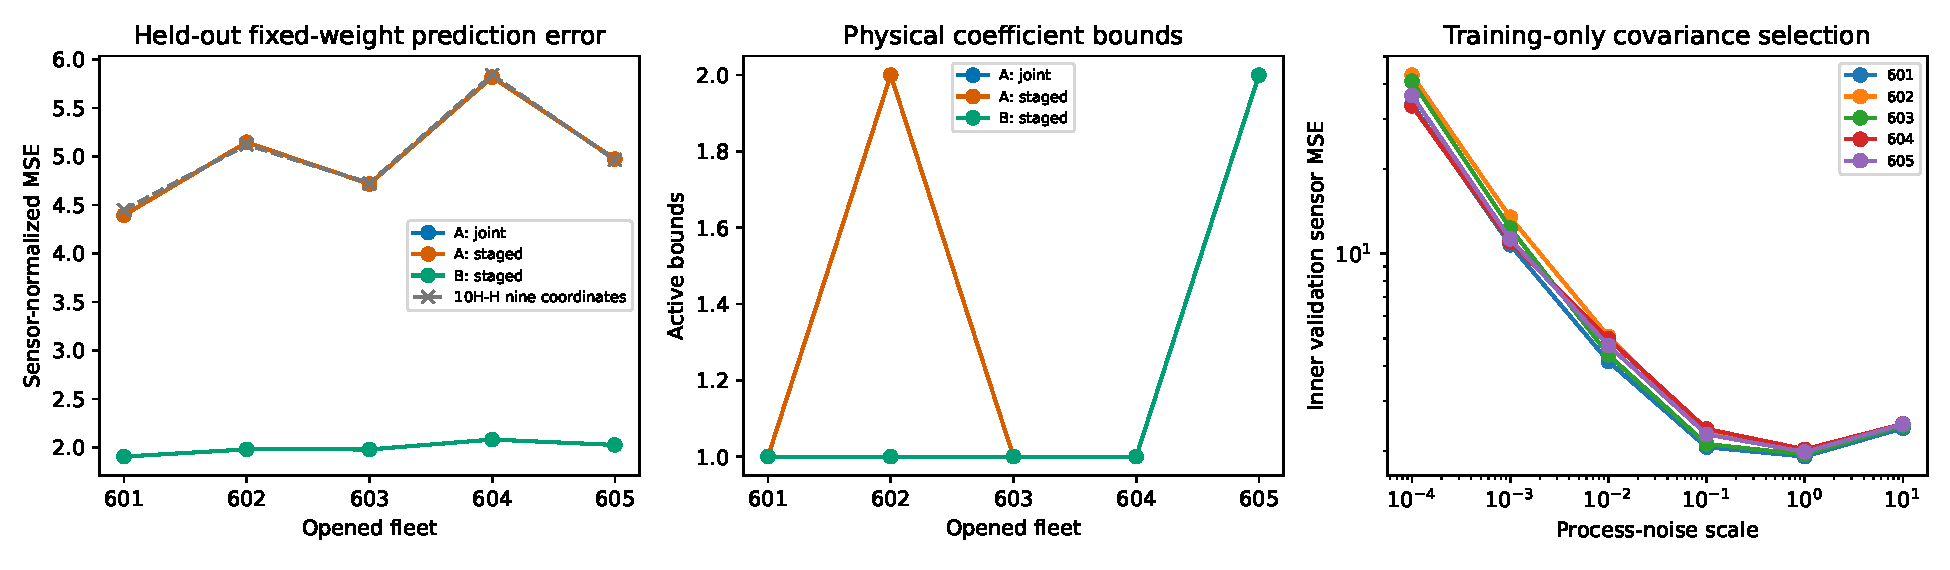
\includegraphics[width=0.98\linewidth]{../results/figures/experiment_10hi_physically_coupled_fit.pdf}
\caption{Absolute held-out prediction error, active coefficient bounds, and
training-only covariance scores. Part A uses the inherited scale; Part B
uses its inner-selected scale. The left panel uses absolute errors to avoid
comparing percentage gains against different nominal covariances.}
\label{fig:10hi-physical-fit}
\end{figure}

\paragraph{Post-hoc innovation calibration.}
A separate measured-output audit leaves models, selections, and gates
unchanged. Correctly specified Gaussian innovations would have unit mean
normalized innovation squared, identity whitened covariance, and no serial
correlation. The fitted Part A models instead have mean normalized NIS
4.013 and maximum absolute lag-one correlation 0.879. Part B reduces these
to 0.445 and 0.346. Its whitened covariance eigenvalues are all below one,
with ranges 0.173--0.183 for the smallest and 0.684--0.728 for the largest.
The prediction-selected covariance therefore produces conservative innovation
variances and leaves appreciable serial structure. Better one-step prediction
does not validate a calibrated likelihood for assigning vehicle groups.
Heterogeneous pooling, the fixed covariance shape, and quiet-bias uncertainty
remain possible contributors. These diagnostics do not isolate their causes.

\paragraph{Decision.}
The eight-coordinate physical relation and the estimator implementation are
validated on the declared development checks. Measured-output prediction
remains useful and final fitting is reproducible. The homogeneous references
recover interior parameters, while heterogeneous pooled fits remain bounded.
This argues against missing physical coupling being the sole explanation for
the earlier boundary solutions. It does not prove that heterogeneity alone
causes them.

The complete physical/covariance gate fails. Joint group/model learning is
still deferred under that gate. The next focused work must resolve the inner
stationarity exception and distinguish predictive covariance tuning from
likelihood calibration, while diagnosing the pooled-model boundary/profile
limitations. Parameter bounds should remain unchanged unless a new public
physical argument justifies a separately declared protocol. These results
do not establish latent-state accuracy, closed-loop improvement, or blind
confirmation performance.

\paragraph{Reproducibility.}
The protocol, learner, runner, and tests were archived before fleet fitting
in commit \texttt{0381587}. The implementation is in
\path{code/src/federated_lpv/physical_coupled_fit.py},
\path{code/experiments/experiment_10hi_physically_coupled_fit.py}, and
\path{code/config/experiment_10hi.json}. Numerical checks cover the exact
mapping, likelihood gradients, information transformation, coupled KKT
normals, feasible nuisance profiles, and client-blocked splits.
Per-fleet CSVs retain parameters, starts, phases, profiles, curvature,
measured-array hashes, inner scores, and covariance selection. No confirmation
execution option exists.
One initial Part A job on seed 602 stopped when a redundant projection of the
zero-offset profile center rejected bound roundoff. Commit \texttt{9f08abc}
reuses the already audited center and resumes that job. The fit, nonzero
profile targets, configuration, and gates are unchanged. An execution manifest
retains the original and corrected runner revisions and their source hashes;
completed jobs were preserved. The innovation audit is explicitly post-hoc.
Validation passes 124 tests and lint, and the full report compiles.
